\documentclass{beamer}

\usepackage[utf8]{inputenc}
\usepackage{default}
\usepackage[italian]{babel}
\usepackage{graphicx}
\usepackage[version=3]{mhchem} % Formula subscripts using \ce{}
\usepackage[style=chem-acs]{biblatex}
\usepackage{leading}

\usetheme{Warsaw}        % layout complessivo. 
\useinnertheme{default} % layout interno.
\useoutertheme{ilario1} % layout esterno.
\usecolortheme{wolverine} % schema di colori.
\usefonttheme{default}  % schema dei font.



\hypersetup{pdfauthor={Ilario Gelmetti},pdfsubject={Plastiche self-healing - Self-healing plastics},pdfkeywords={polymers, plastic, self-healing, mendable, supramolecular},pdftitle={Self-healing plastics}} %metadati nel pdf

\renewcommand{\thefootnote}{} %elimina il numerino della nota a piè di pagina
\renewcommand\footnoterule{}
\setbeamertemplate{navigation symbols}{}

\AtBeginSection[]{\frame{\tableofcontents[current,hideothersubsections] \addtocounter{framenumber}{-1}}} %indice all'inizio di ogni section, mostra solo le sottosezioni di quella sezione

\bibliography{gelmetti-compl_chim_macr-2}

\title{Plastiche auto-riparanti}
\subtitle{Esame di Complementi di Chimica Macromolecolare}
\author{Ilario Gelmetti}
\institute{Scuola Normale Superiore di Pisa.\\Professore Giancarlo Galli.}
\date{23 gennaio 2012}

\begin{document}
\begin{frame}
  \titlepage
\end{frame}




\section{Introduzione}
\section{Introduzione}
\diapo{La chimica del silicio}
Il silicio come ``{\bf traghettatore}'': 
$$\ce{R ->[?] P}$$
$$\ce{R ->C[+Si] I ->[-\ce{Si}] P}$$
\pause
I {\bf legami del silicio}:
\begin{itemize}
 \item {\bf facile rottura} eterolitica da parte di reagenti ionici, {\bf ossigeno e alogeni};
 \item se {\bf legato al carbonio} può essere considerato un {\bf super-protone};
 \item se {\bf legato all'ossigeno} può essere considerato un {\bf protone indebolito}.
\end{itemize}
\end{frame}


%%%%%%%%%%%%%%%%%%%%%%%%%%%%%%%%%%%%%%%%%%%%%%%%%%%%%%%%%%%%%%%%%%%%
\logo{}

\begin{frame}
\frametitle{La chimica del silicio}
\begin{block}{Effetto $\beta$: ($\sigma$--p)$_\pi$}
\begin{figure}{\centering{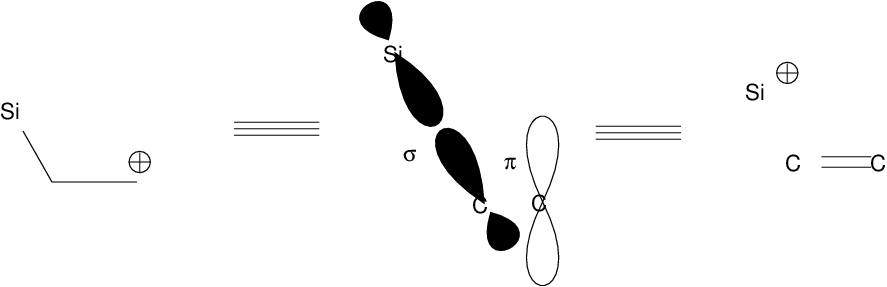
\includegraphics[width=0.7\textwidth]{img/intro/b-effect.png}}}\end{figure}
\end{block}
\pause
\begin{block}{$\alpha$ anioni: ($\sigma$*--p)$_\pi$}
\begin{figure}{\centering{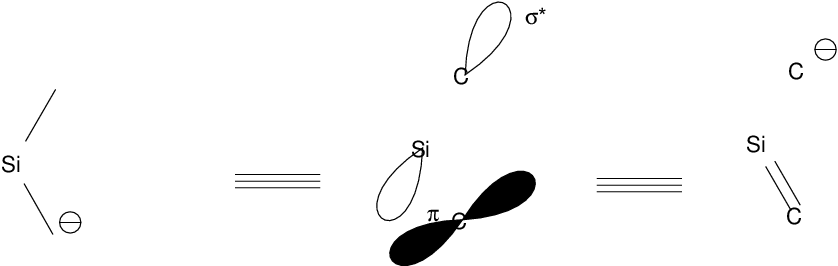
\includegraphics[width=0.7\textwidth]{img/intro/a-anions.png}}}\end{figure}
\end{block}
\end{frame}

\logo{
\includegraphics[width=0.07\paperwidth]{img/snslogo.png}}

%%%%%%%%%%%%%%%%%%%%%%%%%%%%%%%%%%%%%%%%%%%%%%%%%%%%%%%%%%%%%%%%%%%%

\diapo{Schema generale delle reazioni di interesse}
\begin{figure}{\centering{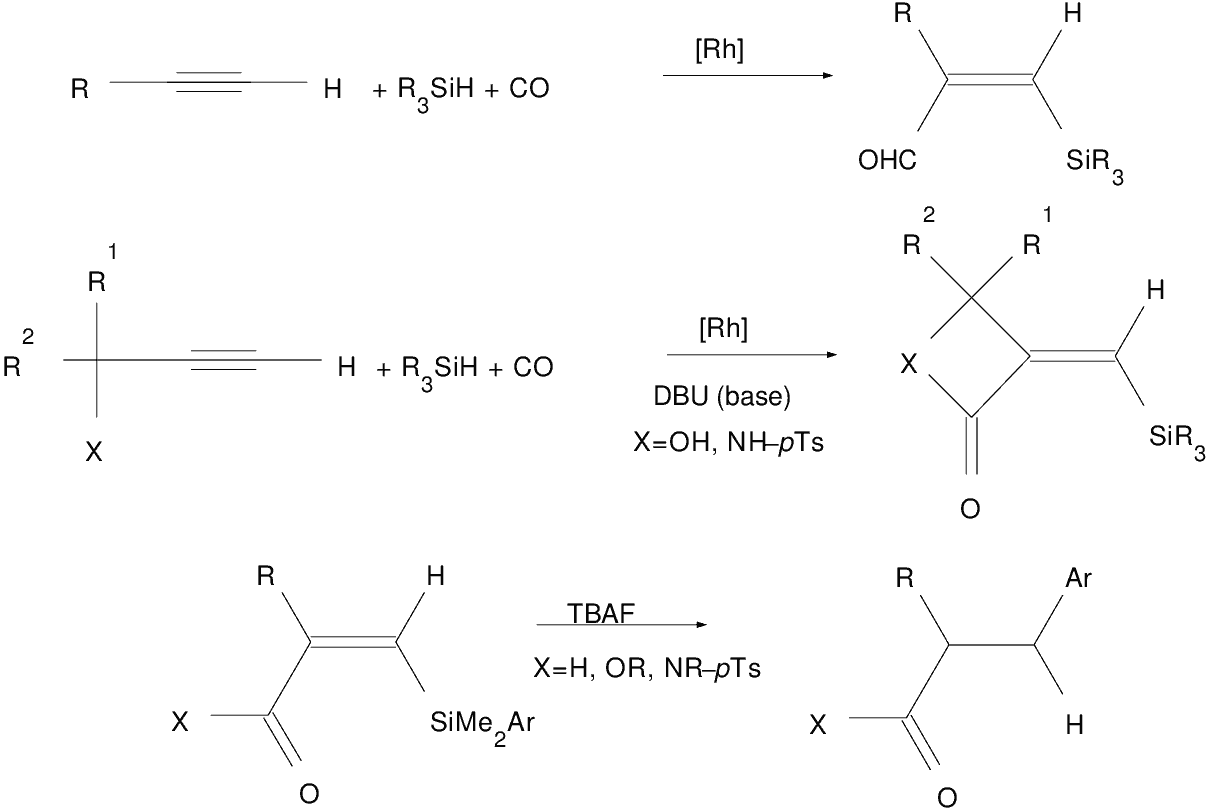
\includegraphics[width=0.8\textwidth]{img/intro/generale.png}}}\end{figure}


\end{frame}

\subsection{Prodotti ottenibili da $\beta$-silil alchenali}\begin{frame}\frametitle{Prodotti ottenibili da $\beta$-silil alchenali}
I $\beta$-sililalchenali ottenuti possono poi essere trasformati sfruttando la {\bf reattività sia di un carbonile $\alpha , \beta $ insaturo sia di un vinil silano}.
\begin{figure}{\centering{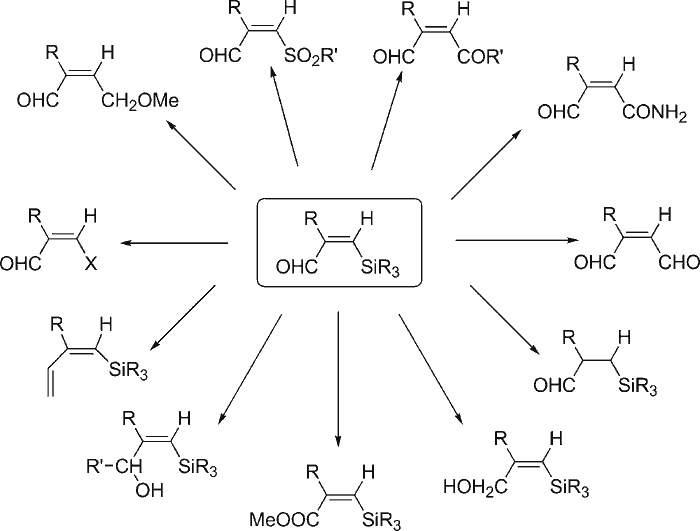
\includegraphics[width=0.6\textwidth]{img/intro/altri_prodotti_ottenibili.png}}}\end{figure}


\end{frame}


%%%%%%%%%%%%%%%%%%%%%%%%%%%%%%%%%%%%%%%%%%%%%%%%%%%%%%%%%%%%%%%%%%%%



\section{Self-healing irreversibile con capsule}

\subsection{Microriserve di materiale polimerizzabile}
\begin{frame}\frametitle{Microriserve di materiale polimerizzabile}
\begin{columns}
 \column{0.65\linewidth}
I \textbf{primi} sistemi self-healing. Viene liberato un \textbf{adesivo liquido} contenuto in: 
\begin{itemize}
 \item microcapsule (poco efficaci);
 \item fibre cave di vetro;
 \item nanotubi di carbonio a singola parete {\tiny(immagine in alto)};
 \item capsule allungate (meno costose);
 \item sistemi microvascolari {\tiny(immagine in basso)}. 
\end{itemize}
Se vengono impiegate fibre o nanotubi per migliorare le proprietà meccaniche, queste rendono il materiale più fragile, perciò è utile il sistema self-healing.

 \column{0.35\linewidth}
\vspace{-13pt}
\begin{figure}{\centering{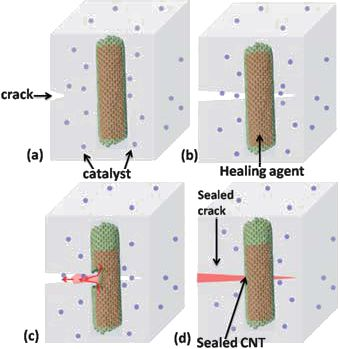
\includegraphics[width=1\textwidth]{irreversibile/nanotubi.jpg}}}\end{figure}\vspace{-13pt}
\begin{figure}{\centering{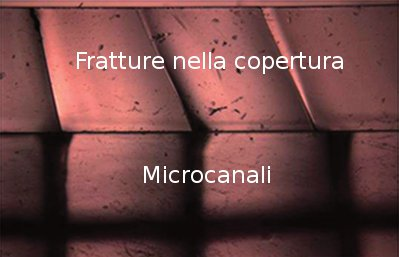
\includegraphics[width=0.7\textwidth]{irreversibile/vascolare.jpg}}}\end{figure}

\end{columns}
\footnote{\tiny \fullcite{irreversibile}}
\end{frame}





\subsection{Capsule contenenti solvente}
\begin{frame}\frametitle{Capsule contenenti solvente}
Il \textbf{solvente} contenuto nelle capsule \textbf{abbassa} la temperatura di \textbf{transizione vetrosa} del materiale \textbf{termoplastico} sotto la temperatura ambiente, si ha riparazione per \textbf{interdiffusione} (\emph{reptation}) delle catene polimeriche tra le facce della frattura.
Questo meccanismo è stato applicato sia in polimeri termoplastici \textbf{sia in termoindurenti}.

\vspace{20pt}

Problema comune a questo ed al precedente metodo: sviluppare \textbf{capsule resistenti} ai processi di estrusione \textbf{ma che si rompano} alla frattura del materiale.


\end{frame}



\section{Self-healing reversibile per legami non covalenti}
\subsection{Polimerizzazione per quadruplo legame ad idrogeno}
\begin{frame}\frametitle{Polimerizzazione per quadruplo legame ad idrogeno}
\begin{columns}
 \column{0.5\linewidth}
Le unità in figura sono autocomplementari ed hanno altissima costante d'associazione. Il materiale in figura in basso ad \textbf{alta temperatura} si comporta come \textbf{fluido} con i monomeri separati, a \textbf{temperatura ambiente} è un \textbf{polimero ad alto peso molecolare}. 
\column{0.5\linewidth}
\begin{figure}{\centering{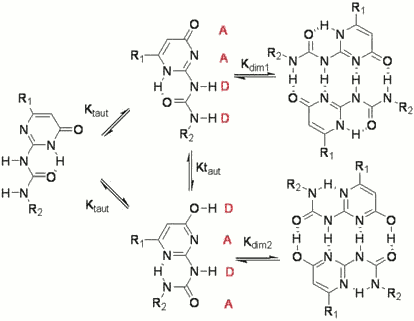
\includegraphics[width=1\textwidth]{legame_h/quadruplo-tautomeri.png}}}\end{figure}
\end{columns}\vspace{-5pt}
\begin{figure}{\centering{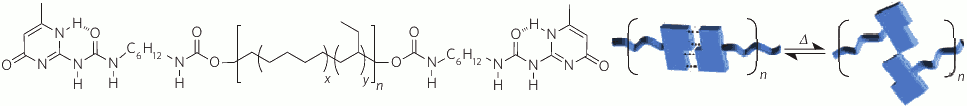
\includegraphics[width=1\textwidth]{legame_h/quadruplo.png}}}\end{figure}\vspace{-20pt}
\footnote{\tiny \leading{5pt} \fullcite{quadruplo} \\ \fullcite{quadruplo-polim}}
\end{frame}

\subsection{Reticolazione per legami ad idrogeno}
\begin{frame}\frametitle{Reticolazione per legami ad idrogeno}

La \textbf{varietà} strutturale \textbf{evita la cristallizzazione} nella \textbf{gomma}.
\begin{columns}
 \column{0.45\linewidth}
I nuclei poliacidi sono dimeri e trimeri di \textbf{acidi grassi} di origine vegetale. Viene plastificato con dodecano. Una volta \textbf{tagliato}, le superfici vanno \textbf{poste in contatto entro breve tempo} per \textbf{evitare} che le coppie spezzate \textbf{si riorganizzino} all'interno delle due superfici. Ha bassa deformabilità.

\column{0.6\linewidth}
\begin{figure}{\centering{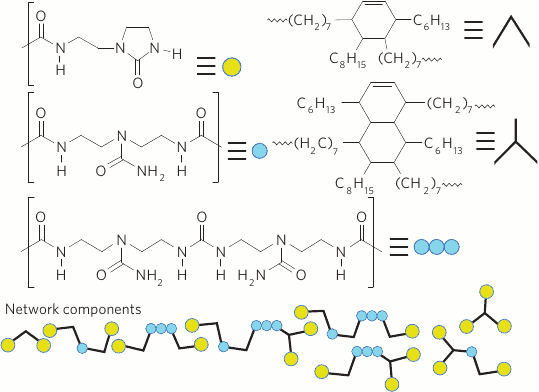
\includegraphics[width=1\textwidth]{legame_h/leibler.png}}}\end{figure}
\end{columns}
\footnote{\tiny \leading{5pt} \fullcite{leibler-nature}\\\fullcite{leibler-sintesi}\\\fullcite{leibler-2010}}
\end{frame}




\subsection{Reticolazione per $\pi-\pi$ stacking}
\begin{frame}\frametitle{Piccole molecole reticolate per  $\pi-\pi$ \emph{stacking}}

Per avere una interazione di \emph{stacking} abbastanza forte è stato usato un \textbf{aromatico elettronricco ed uno elettronpovero} insieme a legami ad idrogeno.

Il materiale presenta una intensa \textbf{colorazione rossa} a causa del trasferimento di carica. 

La \textbf{riparazione} avviene \textbf{perfettamente} ma solo a temperature maggiori di 50$^\circ$C.

\begin{figure}{\centering{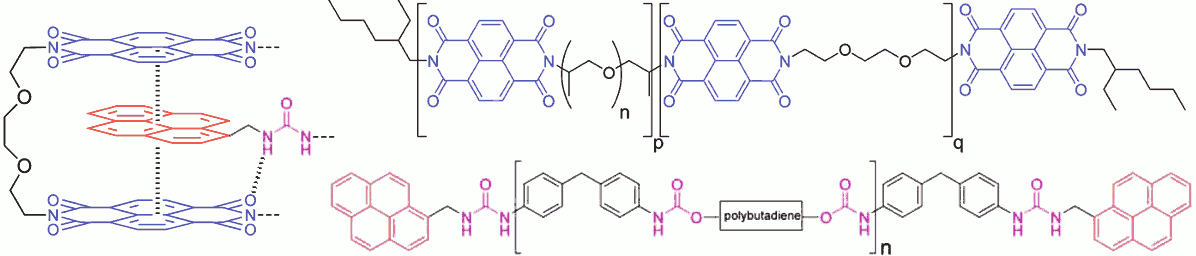
\includegraphics[width=0.9\textwidth]{legame_h/stacking.png}}}\end{figure}\vspace{-10pt}
\footnote{\tiny \leading{5pt} \fullcite{stacking}}
\end{frame}




\subsection{Reticolazione per interazione ionica}
\begin{frame}\frametitle{Reticolazione per interazione ionica}
Gli \textbf{ionomeri} sono \textbf{poli acidi carbossilici neutralizzati} con fino al 15\% eq di \ce{NaOH} aventi \textbf{interazioni} fisiche tra le \textbf{catene laterali ioniche}. 


Quando si ha l'impatto di un \textbf{proiettile} questo porta a \textbf{fusione} il materiale e forma un foro. Dunque il fuso \textbf{chiude elasticamente} il foro, successivamente per \textbf{interdiffusione} avviene la saldatura.  

\footnote{\tiny \leading{5pt} \fullcite{ionomeri}}
\begin{columns}
 \column{0.5\linewidth}
\begin{figure}{\centering{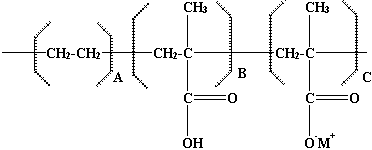
\includegraphics[width=0.9\textwidth]{legame_h/surlyn.png}}}\end{figure}
\column{0.5\linewidth}
\begin{figure}{\centering{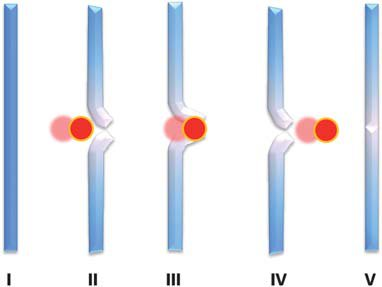
\includegraphics[width=0.6\textwidth]{legame_h/ionomero.jpg}}}\end{figure}
\end{columns}
\end{frame}




\subsection{Altro}
\begin{frame}\frametitle{Altro}
Molti altri sistemi non sono stati trattati, ad esempio:\vspace{-10pt}
\begin{columns}
 \column{0.6\linewidth}
\begin{figure}{\centering{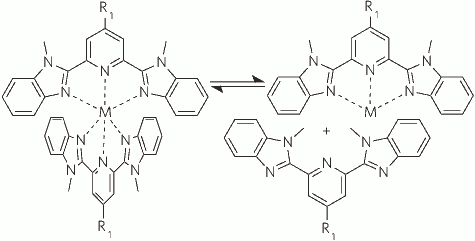
\includegraphics[width=0.8\textwidth]{legame_h/altri-metallo.png}}}\end{figure}
\column{0.4\linewidth}
\begin{figure}{\centering{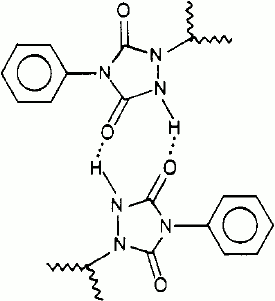
\includegraphics[width=0.4\textwidth]{legame_h/altri-2h.png}}}\end{figure}
\end{columns}
\begin{figure}{\centering{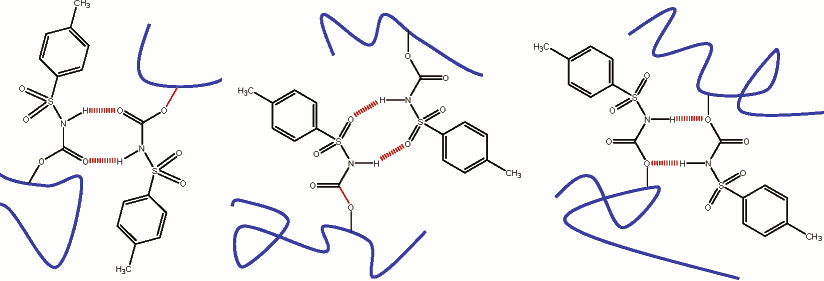
\includegraphics[width=0.9\textwidth]{legame_h/altri-solfo.png}}}\end{figure}

\end{frame}

\section{Self-healing reversibile per legami covalenti}
\subsection{Reticolazione covalente via alcossiammine}
\begin{frame}\frametitle{Reticolazione covalente via alcossiammine}
I polimeri che si basano su interazioni \textbf{non covalenti subiscono deformazioni} permanenti, quelli basati su interazioni \textbf{covalenti diventano dinamici solo se scaldati}.

Nel sistema in figura i \textbf{radicali} formati sono \textbf{stabili} e non reagiscono con altri gruppi funzionali presenti.

Il sistema può essere \textbf{de-reticolato} a caldo in presenza di un \textbf{eccesso di alcossiammina}.
\begin{figure}{\centering{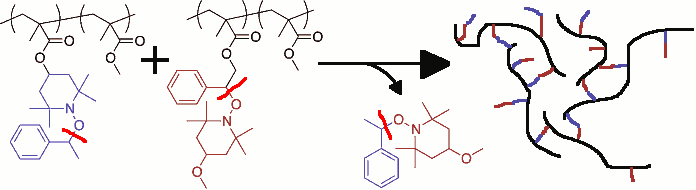
\includegraphics[width=0.9\textwidth]{covalente/alcossiammina.png}}}\end{figure}\vspace{-20pt}
\footnote{\tiny  \fullcite{radicali}}
\end{frame}

\subsection{Reticolazione covalente via Diels Alder}
\begin{frame}\frametitle{Reticolazione covalente via Diels Alder}
\begin{columns}
 \column{0.6\linewidth}
Con la reticolazione covalente reversibile si possono avere \textbf{a temperatura ambiente le proprietà di un termoindurente} (alto modulo elastico, \textbf{1}) \textbf{oppure dinamici a temperatura ambiente} (\textbf{3}). Possono essere in \textbf{singolo componente per evitare lo smescolamento} (\textbf{2}).\vspace{25pt}
\column{0.4\linewidth}\vspace{-10pt}
\begin{figure}{\centering{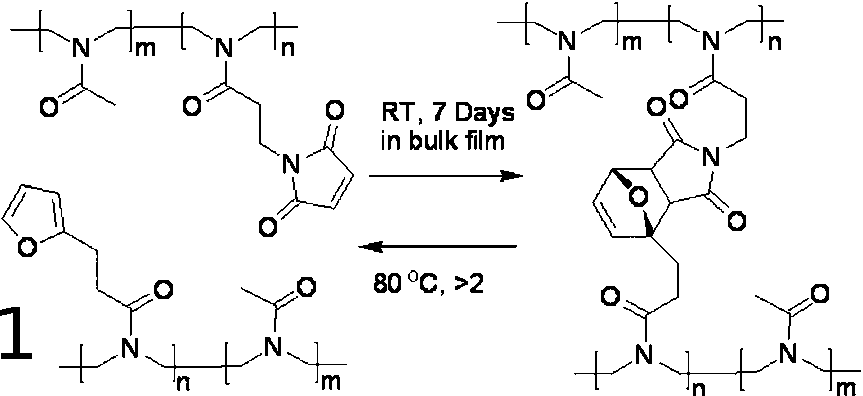
\includegraphics[width=1\textwidth]{covalente/DA.png}}}\end{figure}\vspace{-15pt}
\begin{figure}{\centering{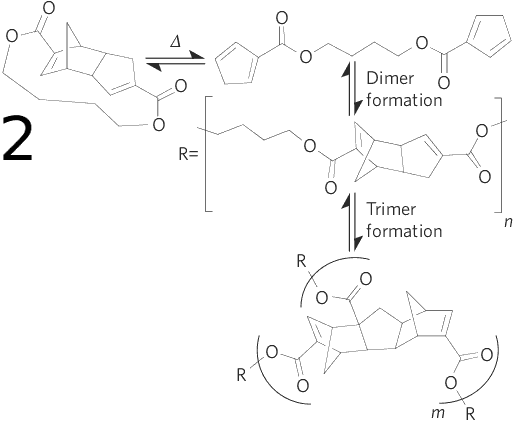
\includegraphics[width=1\textwidth]{covalente/diels-alder1.png}}}\end{figure}

\end{columns}
\vspace{-35pt}
{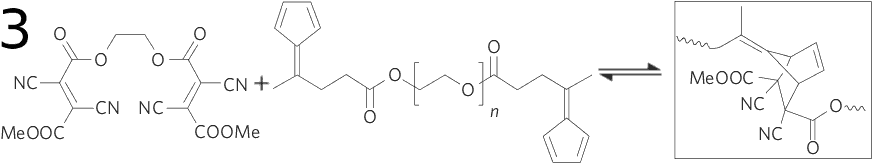
\includegraphics[width=0.8\textwidth]{covalente/diels-alder3.png}}
\footnote{\tiny \leading{3pt} \textbf{1} \fullcite{dielsalder} \textbf{2} \fullcite{dielsalder-dyn} \textbf{3} \fullcite{dielsalder-ram}}

\end{frame}



\subsection{Reticolazione covalente via transesterificazione}
\begin{frame}\frametitle{Reticolazione covalente via transesterificazione}
Questo sistema (a differenza dei precedenti) non si basa su un equilibrio ma su \textbf{reazioni di scambio}, transesterificazioni, dunque \textbf{non sarà disturbato dai solventi}.
Alzando la temperatura, il sistema \textbf{diminuisce in modo graduale la viscosità} passando da solido a fluido viscoso.

La cinetica può essere accelerata introducendo \textbf{catalizzatori inorganici}.
\begin{columns}
 \column{0.8\linewidth}
\begin{figure}{\centering{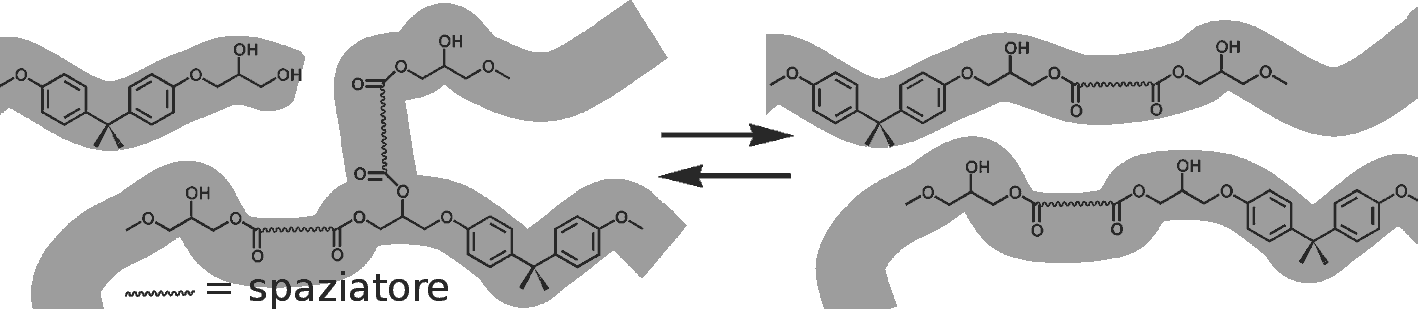
\includegraphics[width=1\textwidth]{covalente/transesterificazione.png}}}\end{figure}
\column{0.2\linewidth}
\begin{figure}{\centering{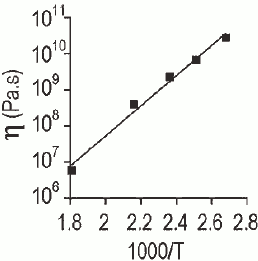
\includegraphics[width=1\textwidth]{covalente/transesterificazione-viscosita.png}}}\end{figure}
\end{columns}
\footnote{\tiny \fullcite{transesterificazione}}
\end{frame}

\subsection{Altro}
\begin{frame}\frametitle{Altro}
\vspace{-5pt}
Molti altri sistemi non sono stati trattati, ad esempio:\vspace{-10pt}
\begin{columns}
 \column{0.5\linewidth}
\begin{figure}{\centering{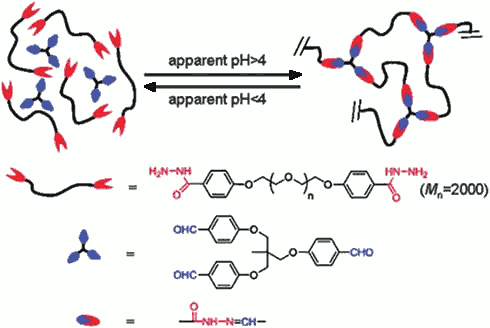
\includegraphics[width=1\textwidth]{covalente/altri-acilidrazone.png}}\\è dinamico}\end{figure}
\vspace{-10pt}\begin{figure}{\centering{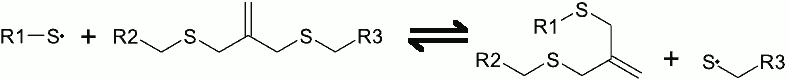
\includegraphics[width=1\textwidth]{covalente/altri-tio.png}}\\la plasticità è fotoindotta}\end{figure}

\column{0.5\linewidth}
\begin{figure}{\centering{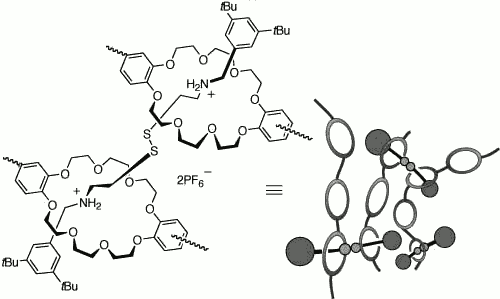
\includegraphics[width=1\textwidth]{covalente/altri-disolf.png}}\\tioli catalizzano l'apertura}\end{figure}

\begin{figure}{\centering{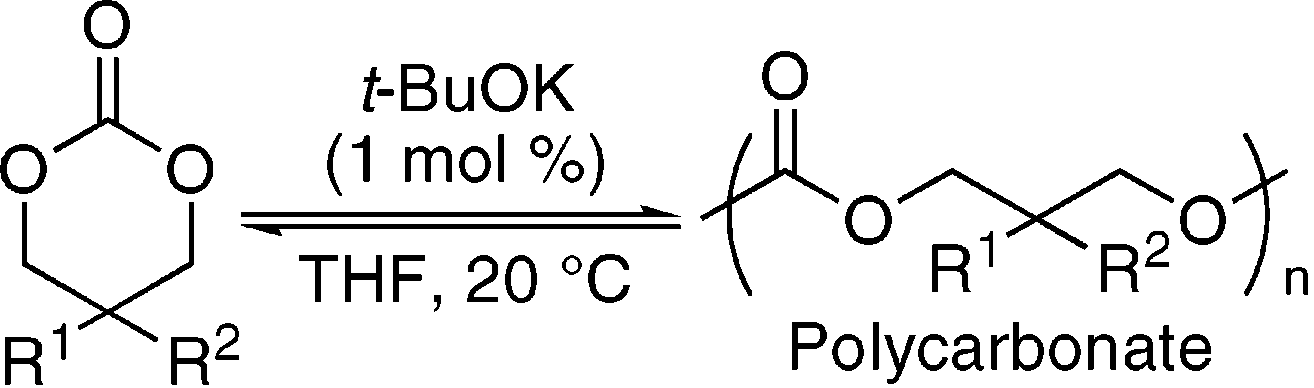
\includegraphics[width=0.7\textwidth]{covalente/altri-carbonato.png}}}\end{figure}

\end{columns}

\end{frame}

\section{Self-healing per altri meccanismi}
\subsection{Riparazione per irraggiamento}
\begin{frame}\frametitle{Riparazione per irraggiamento}
\begin{columns}
 \column{0.65\linewidth}
Il sistema in figura è \textbf{eterogeneo}. 

Probabilmente alla rottura o all'irraggiamento viene \textbf{rotto l'ossetano ed il ponte cerchiato in figura}; si ha poi una \textbf{nuova reticolazione} favorita dall'irraggiamento UV.

La riparazione \textbf{non può ripetersi} nello stesso punto.


 \column{0.35\linewidth}
\begin{figure}{\centering{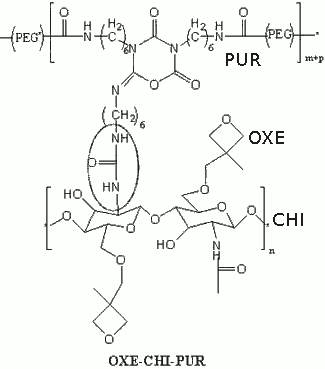
\includegraphics[width=1\textwidth]{altro/oxe-chi-pur.png}}}\end{figure}
\end{columns}
\footnote{\tiny  \fullcite{ottico}}

\end{frame}





\subsection{Riparazione per riscaldamento resistivo}
\begin{frame}\frametitle{Riparazione per riscaldamento resistivo}
\textbf{Scaldando} un filo di materiale \textbf{tramite passaggio di corrente} si ha un \textbf{riscaldamento maggiore} nelle zone in cui sono presenti delle fratture.

Il \textbf{polimero organometallico} riportato in figura è conduttore e può polimerizzare e depolimerizzare facilmente.

Alternative più semplici considerano materiali più comuni rinforzati da \textbf{fibra di carbonio che funge da conduttore}.
\begin{columns}
 \column{0.6\linewidth}
\begin{figure}{\centering{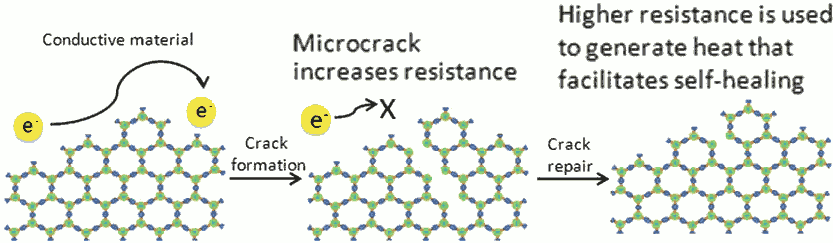
\includegraphics[width=1\textwidth]{altro/resistenza.png}}}\end{figure}
\column{0.4\linewidth}
\begin{figure}{\centering{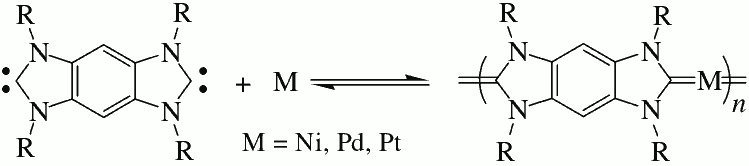
\includegraphics[width=1\textwidth]{altro/metallorganico.png}}}\end{figure}
\end{columns}
\footnote{\tiny  \fullcite{resistenza}}

\end{frame}





\subsection{Riparazione per diffusione di polimeri lineari}
\begin{frame}\frametitle{Riparazione per diffusione di polimeri lineari}

\begin{columns}
 \column{0.5\linewidth}In un polimero termoindurente viene \textbf{dissolto} in piccole quantità \textbf{un polimero termoplastico}.

\textbf{A temperatura ambiente} il polimero termoplastico \textbf{è fissato} al reticolo tramite legami ad idrogeno.

\textbf{Scaldando} e mettendo in contatto due superfici si ha sblocco e \textbf{diffusione} a riparare parzialmente la frattura.


 \column{0.5\linewidth}
\vspace{-13pt}
\begin{figure}{\centering{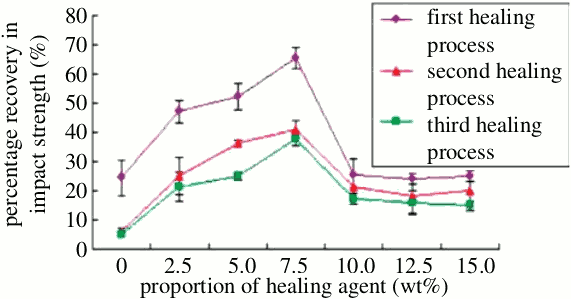
\includegraphics[width=1\textwidth]{altro/diffusione1.png}}}\end{figure}
\vspace{-20pt}
\begin{figure}{\centering{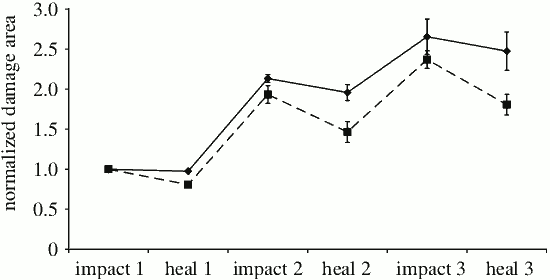
\includegraphics[width=1\textwidth]{altro/diffusione2.png}}}\end{figure}

\end{columns}
\footnote{\tiny  \fullcite{diffusione}}
\end{frame}


\end{document}
